
\section{Apprentissage automatique}


\begin{frame}{Apprentissage automatique}

  Un ensemble d'\textcolor{red}{algorithmes} permettant à une machine d'\textcolor{blue}{apprendre un phénomène} à partir de \textcolor{red}{données}

  \begin{center}
      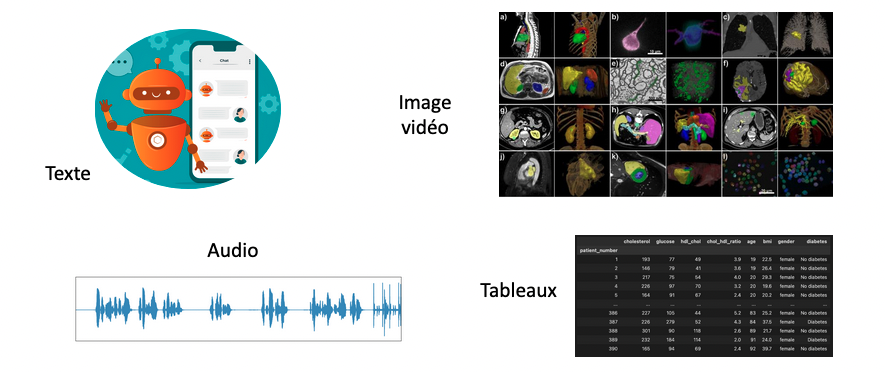
\includegraphics[width=.7\textwidth]{img/ml/multimodal-3.png}
  \end{center}

  \onslide<2>
  Le processus d'apprentissage, souvent via des calculs très longs, donne un \textcolor{orange}{modèle}
\end{frame}


\subsection{Qu'est-ce qu'un modèle ?}


\begin{frame}{Algorithme versus Modèle}

  \textbf{Algorithme}
  
  C'est un \textcolor{red}{ensemble d'opérations} permettant de résoudre une classe de problèmes
  
  Exemple : $98 \times 2 = 100 \times 2 - 4$

  $\longrightarrow$ \textsc{Générique}

  \onslide<2->
  \textbf{Modèle}

  Un modèle est le résultat d'un processus de calcul \textcolor{blue}{adapté aux données}

  \texttt{Modèle = Algorithme + Données}
  
  $\longrightarrow$ \textsc{Spécifique à des données}

  

\end{frame}


\begin{frame}{Exemple du diabète}

  \textbf{Modèle 1}

  Diabète si :
  \begin{itemize}
    \item $\mbox{IMC} > 30$ pour les hommes \only<2>{$\rightarrow$ \alert{70\% de précision}}
    \item $\mbox{IMC} > 25$ pour les femmes \only<2>{$\rightarrow$ \alert{35\% de précision}}
  \end{itemize}

  \begin{overprint}

    \onslide<2>
      \begin{columns}
        \begin{column}{.48\textwidth}
          
          {\scriptsize
          \begin{tabular}{llrl}
            \toprule
            ID &  Gender &   IMC &     Diabetes \\
            \midrule
            40             &    male &  35.1 &  No diabetes \\
            65             &  female &  24.7 &     Diabetes \\
            251            &  female &  26.9 &     Diabetes \\
            257            &    male &  25.5 &     Diabetes \\
            299            &    male &  30.7 &     Diabetes \\
            301            &  female &  36.6 &  No diabetes \\
            \bottomrule
          \end{tabular}}
      
      \end{column}    
      
      \begin{column}{.48\textwidth}
        {
          \scriptsize
          \begin{tabular}{lrr}
            \toprule
                          &  Diabetes &  No          \\
            Male              &           &  diabetes    \\
            \midrule
            IMC $<$ 30    &        16 &          104  \\
            IMC $\geq$ 30 &        10 &           32  \\
            \bottomrule
            Female              &           &      \\
            \midrule
            IMC $<$ 25    &        3 &          48  \\
            IMC $\geq$ 25 &        31 &         146  \\
            \bottomrule
          \end{tabular}

        }
      \end{column}
    \end{columns}

    \onslide<3>
      \bigskip
      \textbf{Modèle 3}

      $$
        \mbox{Diabete} = \mbox{fonction}(\mbox{IMC}, \mbox{Age}, \mbox{Alimentation}, \mbox{etc.})
      $$

      \onslide<4>
      \bigskip
      \textbf{Modèle 2}

      $$
        \mbox{Diabete} = a * \mbox{IMC} + b * \mbox{Age} + c * \mbox{Alimentation} + \dots
      $$
    \end{overprint}

    {\footnotesize IMC = Indice de masse corporelle = $\frac{\text{poids}}{\text{taille}^2}$}


\end{frame}

\begin{frame}{Apprentissage supervisé}

  \begin{center}
    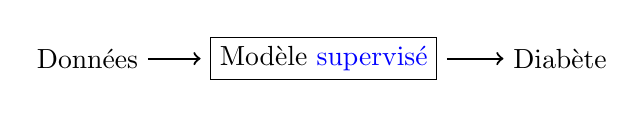
\begin{tikzpicture}[
      every node/.style={align=center},
      arrow/.style={->, thick}
    ]
      \node (table) at (-3,0) {Données};
      
      % Box in the middle
      \node (box) at (0,0) {\fbox{Modèle \textcolor{blue}{supervisé}}};
      
      % Text on the right
      \node (right) at (3,0) {Diabète};
      
      % Arrows
      \draw[arrow] (table) -- (box);
      \draw[arrow] (box) -- (right);
    \end{tikzpicture}
  \end{center}
 
  \bigskip
  Objectif : \textbf{Prédire} un phénomène (le diabète) à partir d'\textbf{observations} (données récoltées sur les patients)
  \bigskip

  \begin{overprint}
    \onslide<1>
  \begin{columns}
    \begin{column}{.48\textwidth}
      \begin{itemize}
        \item \textcolor{red}{Connaissance a priori} de la variable d'intérêt
        \item[\textcolor{white}{x}]
        \item[\textcolor{white}{x}] → Faire le lien entre les observations et la variable d'intérêt
      \end{itemize}
    \end{column}    
    
    \begin{column}{.48\textwidth}
      
      {
        \scriptsize
        \begin{tabular}{llrl}
          \toprule
          ID &  Gender &   IMC &     Diabetes \\
          \midrule
          40             &    male &  35.1 &  No diabetes \\
          65             &  female &  24.7 &     Diabetes \\
          251            &  female &  26.9 &     Diabetes \\
          257            &    male &  25.5 &     Diabetes \\
          299            &    male &  30.7 &     Diabetes \\
          301            &  female &  36.6 &  No diabetes \\
          \bottomrule
        \end{tabular}
      }
    \end{column}
  \end{columns}

\onslide<2>

  \colorwarning{orange} Trois étapes nécessaires :
  \begin{enumerate}
    \item \textcolor{red}{Entrainement} : phase d'apprentissage / construction du modèle
    \item \textcolor{red}{Inférence} : prédiction de nouveaux cas 
    \item Test et \textcolor{red}{évaluation} : estimation de l'erreur commise
  \end{enumerate}

  \end{overprint}



\end{frame}


\begin{frame}{Apprentissage supervisé}
 
  Objectif : \textbf{Identifier} le chiffre manuscrit à partir d'un ensemble d'\textbf{images}
  \bigskip
  \bigskip

  \begin{overprint}
    \onslide<1>
    \begin{center}
      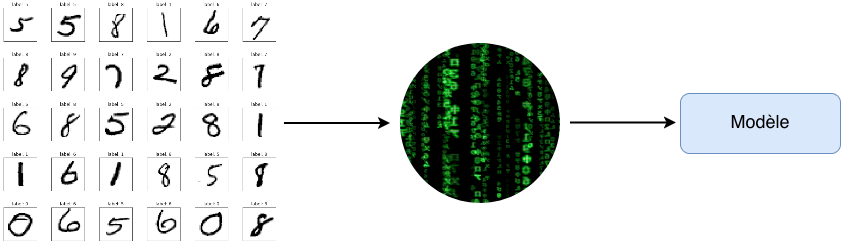
\includegraphics[width=.8\textwidth]{img/mnist_train.png}
    \end{center}

    \onslide<2>
    \begin{center}
      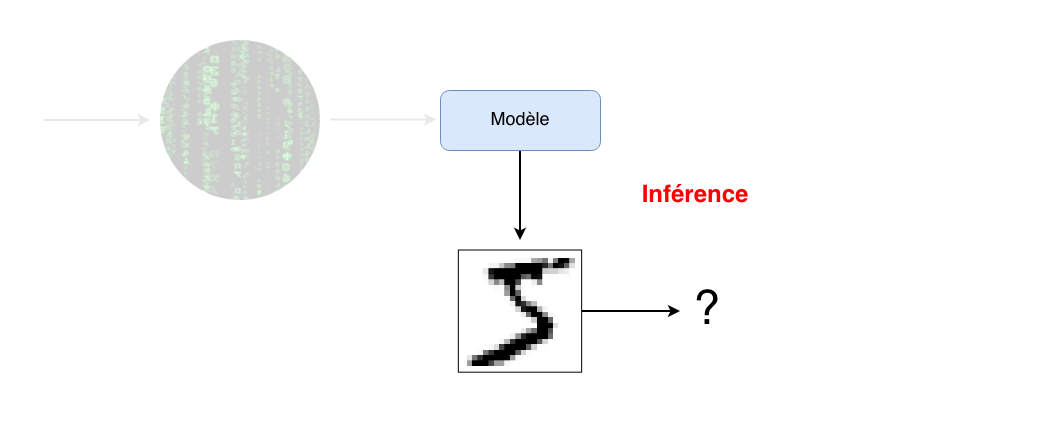
\includegraphics[width=.8\textwidth]{img/mnist_infer_1.png}
    \end{center}
    
    \onslide<3>
    \begin{center}
      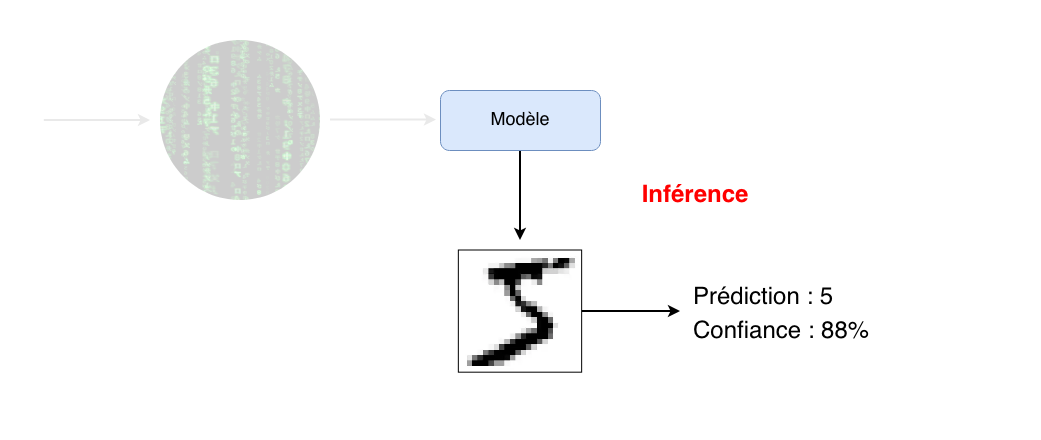
\includegraphics[width=.8\textwidth]{img/mnist_infer_2.png}
    \end{center}
  \end{overprint}
\end{frame}




\begin{frame}{Apprentissage automatique en bref}
  \begin{center}
      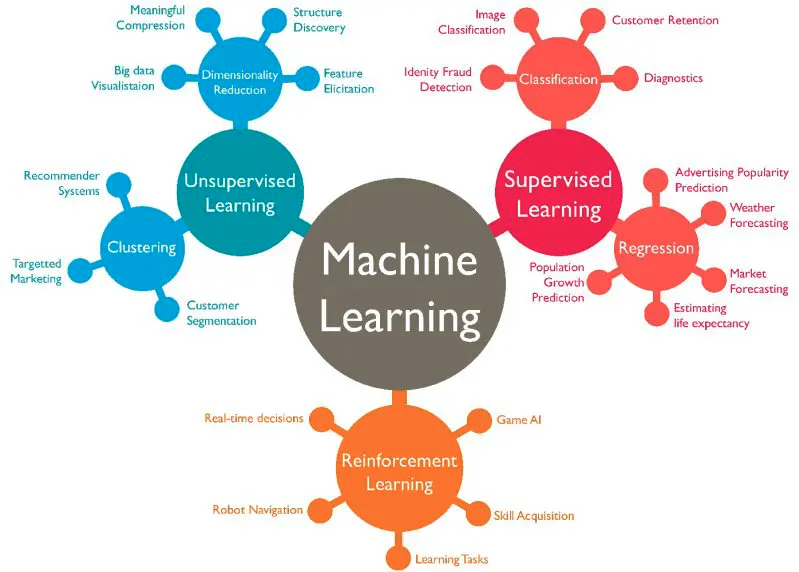
\includegraphics[width=.8\textwidth]{img/ml/ml-algos.png}
  \end{center}
\end{frame}
